\section{Rejouer dans le navigateur}
Après \ui{Simuler}, cliquez sur \ui{Rejouer en 3D}. La scène reprend la hauteur au-dessus du sol et le pas de lecture. Fermer la fenêtre de l'atelier arrête le serveur de cette session.

Le service de dessin prépare l'emprise et les points de passage. Un service distinct de rejeu 3D ouvre une session locale à partir d'un historique existant. Le navigateur reçoit une description de scène JSON et affiche les positions sur une grille de relief, avec une boucle synthétique quand aucun terrain n'est fourni. Le visualiseur Three.js embarqué fournit une caméra orbitale et une vitesse de rejeu réglable. Roassal fournit les couches cartographiques, les observations optiques et les exports PNG et MP4.

\begin{lstlisting}
| scene serveur |
scene := SoSeAtelierRenderScene
    history: simulateur history
    tickSeconds: 1
    terrain: nil
    heightAboveGround: 180
    stride: 10.
serveur := SoSeAtelierRenderServer on: scene.
serveur open.
\end{lstlisting}

Conservez la référence au serveur pour appeler \sel{serveur stop}. Dans une mission géoréférencée, transmettez une instance de \sel{SoSeAtelierTerrain} et la durée de tik réellement utilisée par la simulation. \sel{scene writeTo:} conserve une scène versionnée pour le rejeu.

\begin{figure}[ht]
\centering
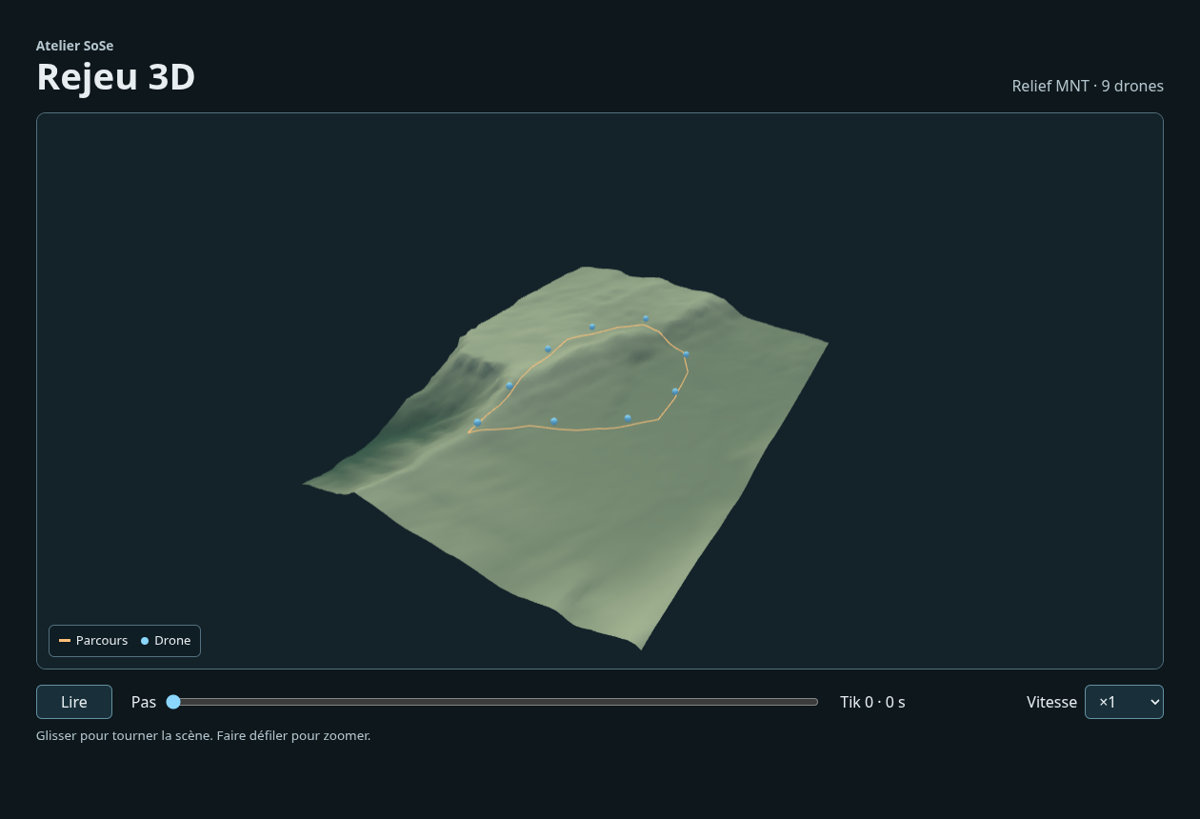
\includegraphics[width=.65\linewidth,height=51mm,keepaspectratio]{rejeu-web.jpg}
\caption{Rejeu Web en 3D d'un historique simulé sur le relief du Vercors. Le navigateur affiche le tracé et la position des drones aux états enregistrés.}
\end{figure}
